%!TEX root = ../diplom.tex

\section{Моделирование отраженного импульса}
\label{sec:pulse_modeling}

Важным преимуществом орбитального радиовысотомера по сравнению с другими радиолокаторами является то, что теоретические модели рассеяния хорошо
описывают свойства радиолокационного сигнала, отраженного морской поверхностью.
В результате алгоритмы обработки получены не с помощью регрессионного анализа,
а основаны на аналитических формулах для формы отраженного импульса.

Если, например, говорить об определении скорости ветра по сечению обратного
рассеяния для скаттерометра, то алгоритмы были получены благодаря применению
регрессионного анализа массива данных, сформированного из контактных измерений
скорости и направления ветра (морские буи) и сечения обратного рассеяния,
измеренного радиолокатором. Погрешность оценки скорости ветра
по сечению обратного рассеяния обусловлена неоднозначностью связи скорости
ветра и сечения обратного рассеяния.

У радиовысотомера при определении с высоты значительного волнения происходит
именно процесс измерения, т.к. существует однозначная связь формы переднего
фронта отраженного импульса и высоты значительного волнения, которая выражается
через известную формулу. В данном точность измерения ограничивается параметрами
радиолокатора, в частности, длительностью излучаемого импульса и частотой
дискретизации.

При измерении расстояния от радиолокатора до среднего уровня морской
поверхности алгоритм также опирается аналитические формулы и модели, например,
учитывает особенности распространения электромагнитного излучения в атмосфере и
ионосфере, что позволяет обеспечить высокую точность.

Благодаря возможности достоверного теоретического  описания рассеяния
электромагнитного излучения взволнованной водной поверхностью, численное
моделирование является эффективным инструментом для моделирования работы
радиовысотомера и отладки алгоритмов обработки. С его помощью можно провести
численный эксперимент и рассмотреть по отдельности и в комплексе влияние
множества факторов, которые вносят вклад в точность измерений.

\subsection{Схема измерения}%
\label{sub:skhema_izmereniia}

Преимущество численного моделирования по сравнению с экспериментом состоит в
том, что достаточно просто провести сравнение различных схем измерения и
оценить их эффективность для решения конкретной задачи. Однако для этого
необходимо подробно описать и перевести в числовую форму все важные для
моделирования параметры схемы измерения. В результате это позволит провести
полноценный <<численный>> эксперимент.  Для описания схемы измерения необходимо
задать угол зондирования (падения) $\theta$, высоту орбиты $H_0$, скорость и
направление движения $v_{rad}$, и направление зондирования $\phi_{rad}$. 

Расстояние от радиолокатора до точки отражения на плоскости $xy$ равно $R_0$ .
Для определенности выберем направление движения радиовысотомера вдоль оси $x$.


Для плоской поверхности формирование отраженного импульса начинается при
касании поверхности передним фронтом падающего импульса в точке непосредственно
под радиовысотомером. Это кратчайшее расстояние от радиовысотомера до
поверхности. На рис.\ref{fig:wave_form} показан пример изменения формы
рассеивающей площадки и формы отраженного импульса в зависимости от времени.
\begin{figure}[h]
    \centering
    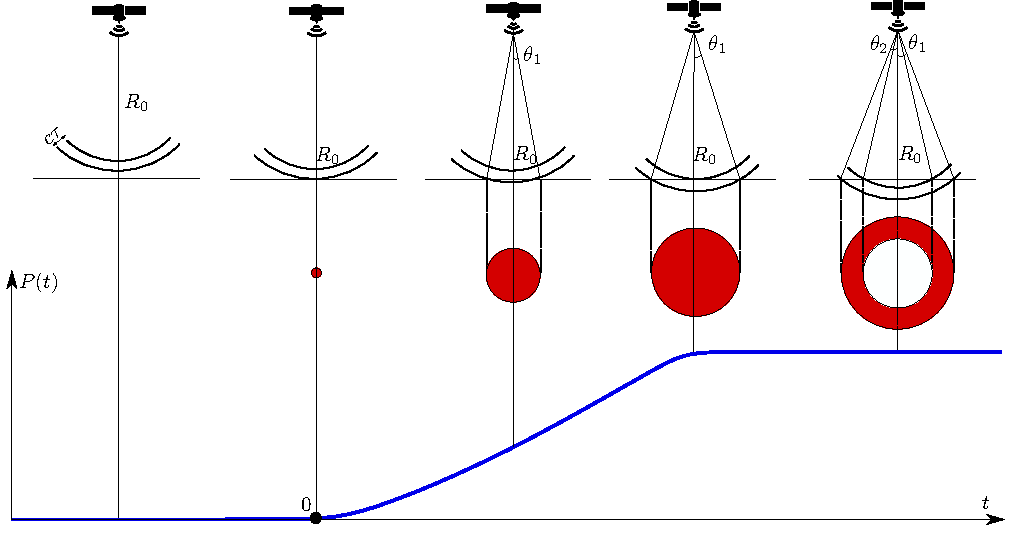
\includegraphics[]{fig/flat_wave1.pdf}
    \caption{Процесс формирования отраженного импульса в зависимости от времени}
    \label{fig:wave_form}
\end{figure}

Для нахождения отраженного импульса необходимо выполнить интегрирование по
рассеивающей площадке для сферической волны с учетом длительности зондирующего
импульса.


\subsection{Влияние морского волнения на форму отраженного импульса}%
\label{sub:vliianie_morskogo_volneniia_na_vormu_otrazhennogo_impul_sa}

Если говорить о морской поверхности, то перед интегрированием по рассеивающей
площадке необходимо выяснить какие участки поверхности будут вносить свой вклад
в формирование отраженного импульса.  При малых углах падения механизм обратного  рассеяния является квазизеркальным и отражение происходит на участках волнового профиля, ориентированных
перпендикулярно падающему излучению. Тогда в формировании отраженного сигнала
будут участвовать только площадки, ориентированные нормально к излучению. 
Поэтому для моделирования рассеяния нам необходимо знать не только высоту
в выбранной точке точке, но и уравнение касательной к ней плоскости, другими словами необходимо знать наклоны $\zeta_x$ и  $\zeta_y$ в искомой точке.

%\footnote{Под словосочетанием <<отражающая точка>> подразумевается
    %физически малая отражающая площадка с большим радиусом кривизны, по которой
%во время вычисления отраженного поля производится интегрирование}. 

Зная координаты радиолокатора  $(x_0,y_0,z_0)$, координаты точки на
поверхности $(x,y,z)$ и наклоны в этой точке $(\zeta_x,\zeta_y,1)$, можем из
геометрии (см. рис. \ref{fig:local_theta}) получить локальный угол падения
волны на морскую поверхность $\theta_0$:
\begin{equation}
    \label{eq:local_theta}
    \cos \theta_0 =  \frac{\vec R \vec n}{|\vec R| |\vec n|}, \text{ где}
\end{equation}
$R$ -- расстояние от радиолокатора до отражающей точки точки,
 $\vec n$ -- нормально касательной плоскости, проведенной к отражающей точке.
 В случае численного моделирования, когда мы хотим решить задачу нахождения
 формы отраженного импульса от известной морской поверхности, можем найти
 $\vec R$ как
 \begin{equation}
     \label{eq:R_1}
     \vec R = \vec R_0 + \zeta_x \vec n_z,
 \end{equation}




Вероятность того, что угол $\theta_0$ будет точно равен нулю и произойдет
зеркальное отражение для случайной выбранной точки очень мала, поэтому имеет
смысл рассматривать квазизеркальное отражение и вводить ограничение на
максимально допустимый локальный угол отражения. 

Нахождение всех зеркальных точек на характерном пятне радиолокатора  $5\times
5 \text{ км}^2$ представляет собой ресурсоемкую задачу. Но поскольку формирование
импульса носит статистический характер, то мы можем ограничится лишь выборкой зеркальных точек. 




\begin{figure}[h!]
    \centering
    \def\svgwidth{0.75\linewidth}
    \includesvg{local_theta}
    \caption{Геометрия определения локального угла падения. Красной линией
    обозначена касательная плоскость к рассматриваемой отражающей точке
$(x,y,\zeta)$}
    \label{fig:local_theta}
\end{figure}


Теперь, для вычисления поля вблизи приемной антенны радиолокатора нам
необходимо просуммировать отраженное от квазизеркальных точек поле.


Запишем скалярное поле, излучаемое антенной радиолокатора в зеркальную точку с радиус-вектором $\vec
r$
\begin{equation}
    E_{s}(\vec r,t) = \frac{E_0}{r}  \cdot  e^{i(\omega t - \vec k \vec
    R)} U(t)G(\theta), 
\end{equation}
где $U(t)$ -- некоторая функция, ограничивающая длительность импульса,
$G(\theta)$ -- диаграмма направленности антенны.



Тогда вблизи приемной антенны амплитуду поля $E$ можно записать как
\begin{equation}
    \label{eq:E}
    E =  \frac{E_0}{R^2} \exp{-2i\vec k\vec R} \sigma^o 
    G^2(\theta)
    , \text{ где}
\end{equation}
$\sigma^o$ -- сечение обратного рассеяния площадки.

В численном моделировании сложно быстро оценить мощность каждой отдельно взятой
площадки, но в соответствии с \cite{bass-and-fuks} при малых углах падения
эффективно работает метод Кирхгофа и сечение обратного рассеяния $\sigma^o$
можно найти по формуле
 \begin{equation}
     \label{eq:frenel}
     \sigma^o = \frac{\abs{F(0)}^2}{2\cos^4\theta \sqrt{\sigma^2_{yy}\sigma^2_{xx}}}
     \cdot \exp{-\frac{-\tan^2 \theta}{2 \sigma^2_{xx}}},
 \end{equation}
 где $\sigma_{xx}^2$, $\sigma_{yy}^2$ -- дисперсии наклонов вдоль оси $x$ и $y$
 соответственно, вычисляемые по модельной реализации, $F(0)$ -- коэффициент
 Френеля,  $\theta$ -- угол падения на рассеивающую площадку. 


Остается только проинтегрировать уравнение \eqref{eq:E} по всем отражающим
точкам 

\begin{equation}
    E \sim \sum\limits_{i=1}^{M} \frac{E_0}{R_i^2} \exp{-2ikR_i}
    G^2(x,y,\theta_0)
\end{equation}
где $M$ -- количество точек,  $x_i,y_i$ -- координаты  $i-$ой отражающей точки,
 $R_i$-- расстояние от спутника до  $i-$ой точки.


 Результирующая мощность импульса будет равна
 \begin{equation}
     P(t) = \frac{EE^*}{2}
 \end{equation}
 \begin{figure}[h]
     \begin{subfigure}{.55\linewidth}
         \centering
         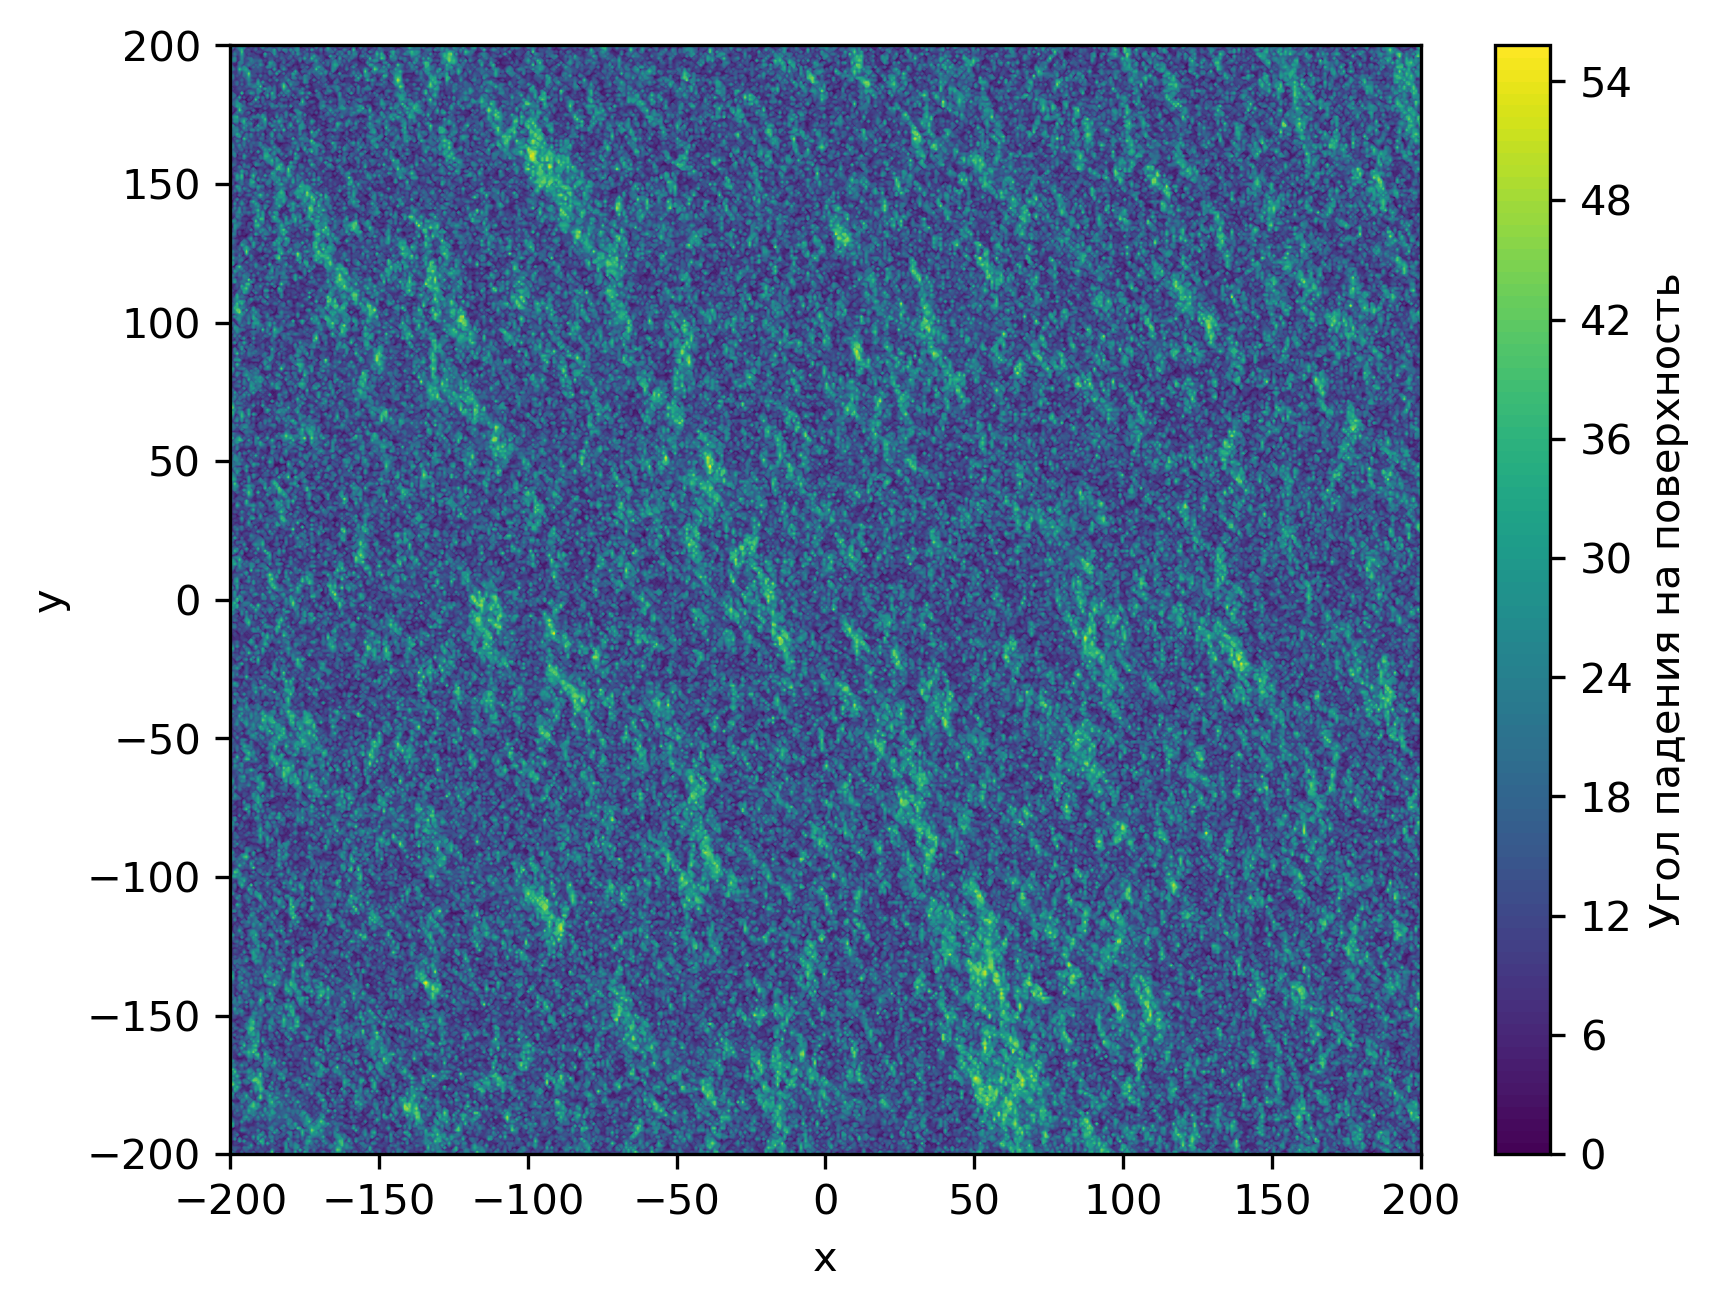
\includegraphics[width=\linewidth]{img/theta0}
         \caption{}
     \end{subfigure}
     \hfill
     \begin{subfigure}{.45\linewidth}
         \centering
         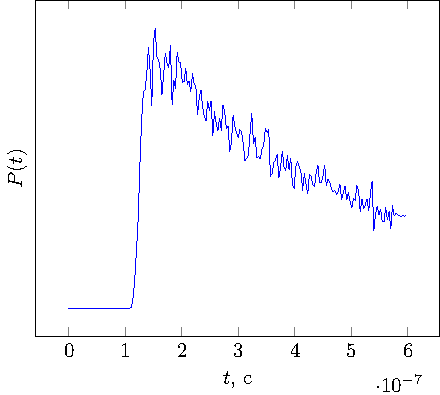
\includegraphics[width=\linewidth]{fig/theta}
         \caption{}
     \end{subfigure}
     \caption{(a) Вычисление локального угла падения (см.\eqref{eq:local_theta}
         )для радиовысотомера, находящегося в точке c координатами $(0,0)$ на
         высоте 1000 км над уровнем моря.  Точки, градусная мера которых меньше
         $\theta<1^\circ$ в дальнейшем будут считаться зеркальными и они будут
         участвовать в формировании отраженного импульса.  (b) Форма
     отраженного импульса в зависимости от времени.}
    \label{fig:model_impuls}
 \end{figure}


 На рис. \ref{fig:model_impuls} изображен модельный импульс, полученный
 суммированием отраженной мощности от выборки зеркальных точек на модельной
 поверхности. 

 Теперь нам необходимо обосновать теоретически полученный импульс и проверить
 как соотносится этот модельный импульс с импульсами, полученными реальными
 спутниками. 

 Об этом и пойдет речь в следующем разделе.
